
\documentclass[10pt]{beamer}
\usepackage{amsmath}
\usepackage{mathtools}
\usepackage{multimedia}
\usepackage{hyperref}


\usefonttheme{professionalfonts} % using non standard fonts for beamer
\usefonttheme{serif} % default family is serif
%\documentclass[12pt]{beamerthemeSam.sty}
\usepackage{epsf}
%\usepackage{pstricks}
%\usepackage[orientation=portrait,size=A4]{beamerposter}
\geometry{paperwidth=160mm,paperheight=120mm}
%DT favorite definitions
\def\LL{\left\langle}	% left angle bracket
\def\RR{\right\rangle}	% right angle bracket
\def\LP{\left(}		% left parenthesis
\def\RP{\right)}	% right parenthesis
\def\LB{\left\{}	% left curly bracket
\def\RB{\right\}}	% right curly bracket
\def\PAR#1#2{ {{\partial #1}\over{\partial #2}} }
\def\PARTWO#1#2{ {{\partial^2 #1}\over{\partial #2}^2} }
\def\PARTWOMIX#1#2#3{ {{\partial^2 #1}\over{\partial #2 \partial #3}} }

\def\rightpartial{{\overrightarrow\partial}}
\def\leftpartial{{\overleftarrow\partial}}
\def\diffpartial{\buildrel\leftrightarrow\over\partial}

\def\BC{\begin{center}}
\def\EC{\end{center}}
\def\BN{\begin{enumerate}}
\def\EN{\end{enumerate}}
\def\BI{\begin{itemize}}
\def\EI{\end{itemize}}
\def\BE{\begin{displaymath}}
\def\EE{\end{displaymath}}
\def\BEA{\begin{eqnarray*}}
\def\EEA{\end{eqnarray*}}
\def\BNEA{\begin{eqnarray}}
\def\ENEA{\end{eqnarray}}
\def\EL{\nonumber\\}

\newcommand{\etal}{{\it et al.}}
\newcommand{\gbeta}{6/g^2}
\newcommand{\la}[1]{\label{#1}}
\newcommand{\ie}{{\em i.e.\ }}
\newcommand{\eg}{{\em e.\,g.\ }}
\newcommand{\cf}{cf.\ }
\newcommand{\etc}{etc.\ }
\newcommand{\atantwo}{{\rm atan2}}
\newcommand{\Tr}{{\rm Tr}}
\newcommand{\dt}{\Delta t}
\newcommand{\op}{{\cal O}}
\newcommand{\msbar}{{\overline{\rm MS}}}
\def\chpt{\raise0.4ex\hbox{$\chi$}PT}
\def\schpt{S\raise0.4ex\hbox{$\chi$}PT}
\def\MeV{{\rm Me\!V}}
\def\GeV{{\rm Ge\!V}}

%AB: my color definitions
%\definecolor{mygarnet}{rgb}{0.445,0.184,0.215}
%\definecolor{mygold}{rgb}{0.848,0.848,0.098}
%\definecolor{myg2g}{rgb}{0.647,0.316,0.157}
\definecolor{A}{rgb}{1.0,0.3,0.3}
\definecolor{B}{rgb}{0.0,1.0,0.0}
\definecolor{C}{rgb}{1.0,1.0,0.0}
\definecolor{D}{rgb}{0.5,0.5,1.0}
\definecolor{E}{rgb}{0.7,0.7,0.7}
\definecolor{abtitlecolor}{rgb}{1.0,1.0,1.0}
\definecolor{absecondarycolor}{rgb}{0.0,0.416,0.804}
\definecolor{abprimarycolor}{rgb}{1.0,0.686,0.0}
\definecolor{Red}           {rgb}{1,0.4,0.4}
\definecolor{Yellow}           {rgb}{1,1,0.0}
\definecolor{Grey}          {cmyk}{.7,.7,.7,0}
\definecolor{Blue}          {cmyk}{1,1,0,0}
\definecolor{Green}         {cmyk}{1,0,1,0}
\definecolor{Brown}         {cmyk}{0,0.81,1,0.60}
\definecolor{Silver}        {rgb}{0.95,0.9,1.0}
\definecolor{Sky}           {rgb}{0.07,0.0,0.2}
\definecolor{Darkbrown}     {rgb}{0.4,0.3,0.2}
\definecolor{40Gray}        {rgb}{0.4,0.4,0.5}
\usetheme{Madrid}


\setbeamercolor{normal text}{fg=Silver,bg=Sky}

%AB: redefinition of beamer colors
%\setbeamercolor{palette tertiary}{fg=white,bg=mygarnet}
%\setbeamercolor{palette secondary}{fg=white,bg=myg2g}
%\setbeamercolor{palette primary}{fg=black,bg=mygold}
\setbeamercolor{title}{fg=abtitlecolor}
\setbeamercolor{frametitle}{fg=abtitlecolor}
\setbeamercolor{palette tertiary}{fg=white,bg=Darkbrown}
\setbeamercolor{palette secondary}{fg=white,bg=absecondarycolor}
\setbeamercolor{palette primary}{fg=white,bg=40Gray}
\setbeamercolor{structure}{fg=abtitlecolor}

\setbeamerfont{section in toc}{series=\bfseries}

%AB: remove navigation icons
\beamertemplatenavigationsymbolsempty
\title[The seasons]{
  \textbf {The seasons}
}

\author [Astronomy 101]{Astronomy 101\\Syracuse University, Fall 2019\\Walter Freeman}

\date{\today}

\begin{document}



\frame{\titlepage}


\frame{
\Huge
\BC
Winter is coming.
\bigskip
\bigskip
\bigskip
\bigskip
\EC
\large
\begin{flushright}---Watchwords of House Stark \\({\it A Song of Ice and Fire}, George R. R. Martin)\end{flushright}}




\frame{

\Huge
\BC
Winter is coming.
\bigskip
\bigskip
\bigskip
\bigskip
\EC
\large
\begin{flushright}---Syracusians, as we buy snow tires and 50 pound bags of salt\end{flushright}
}


\frame{\frametitle{\textbf{Announcements}}
\Large

\begin{itemize}
	\item Friday 8AM lab (TA didn't show up, I covered):
	\begin{itemize}
		\item All students, even those who left early, will get full credit
		\item Any students who stayed and completed the lab will get extra credit
		\item In general, if a TA isn't there on time, please send a Slack message to \#ast101 and @ me
	\end{itemize}

\bigskip
	\item Remember, if you need to miss a lab, talk to lab TA's -- they can help you
	
\end{itemize}
}

\frame{\frametitle{\textbf{Seasonal stars}}
	\Large
\begin{itemize}
	\item The Earth moves around the Sun, so:
	\begin{itemize}
		\item Some stars may be invisible during part of the year, since they are only above the horizon when the Sun also is
		\item Those constellations that lie along the plane of Earth's orbit are called the {\it zodiac}
		\item Astrology (claims to) care about which constellation is ``behind'' the Sun, even though we can't see it
	\end{itemize}
\end{itemize}
}

\frame{
	\Large
	\begin{columns}
		\column{0.5\textwidth}
		Which image shows the position of the Earth {\it \bf exactly} one day later?
		\column{0.5\textwidth}
		\BC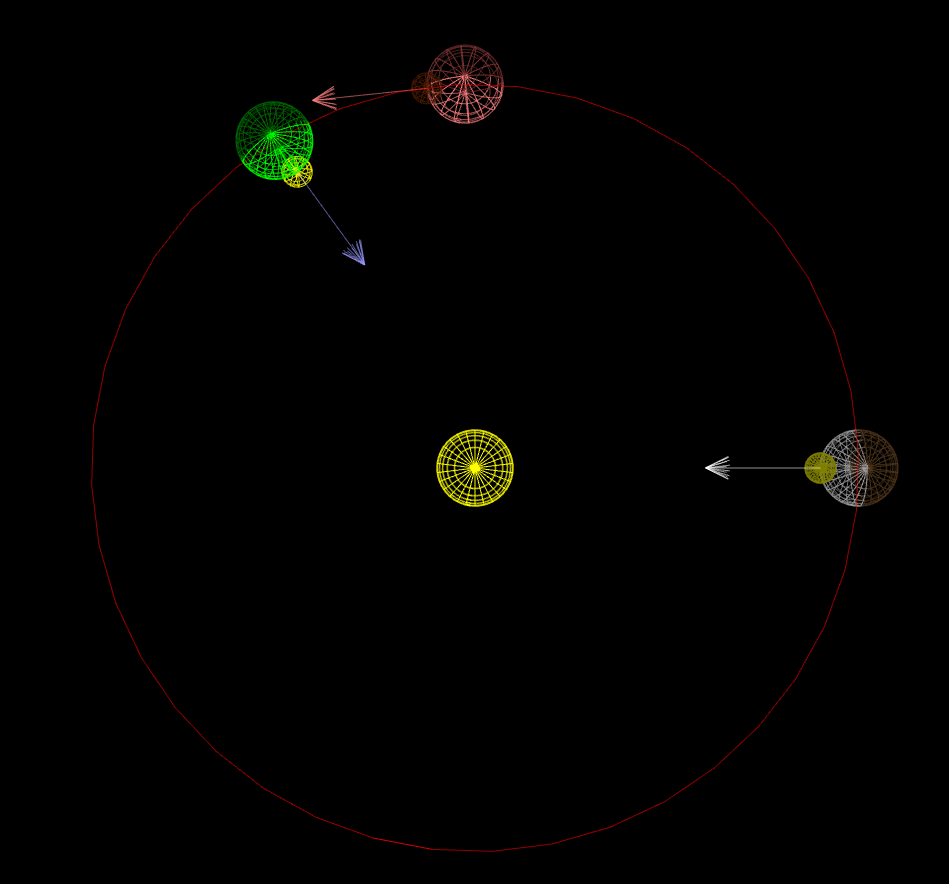
\includegraphics[width=0.9\textwidth]{day-question-1.png}\EC
	\end{columns}
	
	\bigskip
	\bigskip
	
	\color{A}A: The red one \\
	\color{B}B: The green one \\
	\pause
	\color{C}C: Depends on what you mean by ``a day'' \\	
}

\frame{
	\Large
	There are {\it two kinds} of day!
	
	\BI
	\item{Solar day: judged by the position of the Sun}
	\item{Sidereal day (sih-dee-ree-al): judged only by the rotation of the Earth with respect to the stars}
	\EI
	
	Why are they different?
}

\frame{\frametitle{\textbf {Two sorts of day}}
	\large
	The {\it sidereal day} is the amount of time it takes the Earth, and thus the celestial sphere, to rotate once.
	
	\bigskip
	
\BC	{\color{Red} One sidereal day $\rightarrow$ $360^\circ$ rotation of the Earth}\EC
	
\bigskip
\bigskip
    The {\it solar day} is the amount of time from solar noon to solar noon.
    
    \bigskip
    
    Since the Earth orbits the Sun, this requires more than $360^\circ$ rotation:
    \BI
    \item{$360^\circ$ plus a little extra, to compensate for the motion of the Earth around the Sun}
    \item{In my animation, with the ``fast orbit'', this is a lot more than $360^\circ$}
    \item{In the real world, the Earth moves only 1/365 $\approx$ $1^\circ$ around the Sun each day}
    \item{... so in a solar day the Earth rotates:}
    \begin{itemize}
    	\item $360^\circ$ for the stars to rise and set once...
    	\item ... plus {\it one more degree} to compensate for the Earth's movement
    \end{itemize}
    

    
    \EI
\BC   	{\color{Green} One solar day $\rightarrow$ $361^\circ$ rotation of the Earth}    \EC
    
}

\frame{
	
	\begin{columns}
		\column{0.5\textwidth}
		\color{Green}
		\begin{center}
\Large			Solar day:
		\end{center}
		\begin{itemize}
			\normalsize
			\item Exactly 24 hours
			\item $361^\circ$ rotation of Earth
			\item The Sun returns to its same position (east/west)
			\item A bit more than a sidereal day $\rightarrow$ the stars move ``too far''
		\end{itemize}
\column{0.5\textwidth}
\color{Red}
\begin{center}
	\Large			Sidereal day:
\end{center}
\begin{itemize}
	\normalsize
	\item Four minutes less than 24 hours
	\item $360^\circ$ rotation of Earth
	\item The stars return to their same positions (exactly)
	\item A bit less than a solar day $\rightarrow$ the Sun moves ``too little'' 
\end{itemize}
	\end{columns}
}



\frame{\frametitle{\textbf{Finishing from last time}}
\Large Did you finish Lecture Tutorials pp. 11-12 (solar/sidereal day?)

\bigskip
\bigskip
\bigskip
\color{A}A: Yes \\
\color{B}B: Mostly\\
\color{C}C: No 
}

\frame{
	\BC
\Huge Work on {\it Lecture Tutorials} pp. 11-12 if you didn't finish them, and 12-15 \\(parts 1 and 2).
\EC

}

\frame{\frametitle{\textbf{What is a common incorrect explanation for why we have seasons?}}
	
	\huge Send a slack message to \#ast101, and/or react to your classmates' messages.
	
}


\frame{\frametitle{\textbf{The tilt of the Earth's axis}}
\BC\Large
The Earth's axis of rotation is not lined up with its orbital axis. \\

\bigskip

It's tilted by 23.4 degrees.

\bigskip

The axis of rotation changes {\color{Red}only very slowly} (over millennia).

\EC

\bigskip
\bigskip

\BC
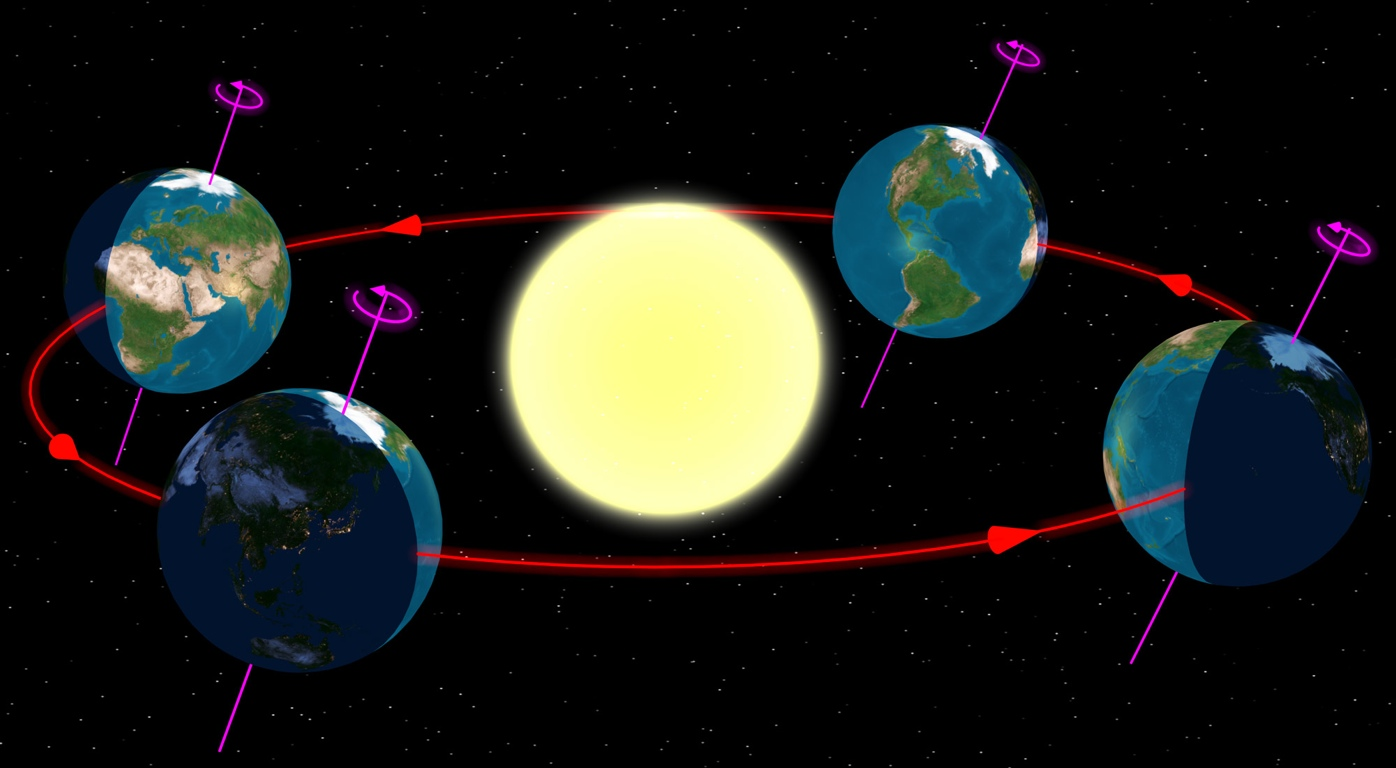
\includegraphics[width=0.8\textwidth]{axial-tilt.jpg}
\EC
}

\frame{\frametitle{\textbf{Let's look at this in animations}}

}


\frame{\frametitle{\textbf{What consequences does this have for the sky?}}

\Large

As the year progresses, thinking only about noon, will the Sun:

\Large

\bigskip
\bigskip
\bigskip

I. Move higher and lower in the sky \\
II. Move east/west relative to the stars

\bigskip
\bigskip
\bigskip

\Huge

\color{A}A: I only \\
\color{B}B: II only \\
\color{C}C: I and II \\
\color{D}D: None of the above 

}


\frame{\frametitle{\textbf{A demonstration in Stellarium}}
\Large
Let's use {\it Stellarium} to examine the Sun at different times of year.

\bigskip
\bigskip
\bigskip


Notice:
\BI
\item{The Sun is higher or lower in the sky depending on the time of year}
\item{The Sun moves westward with respect to the stars:} 
\BI
\item{Every {\it solar day}, the Sun's east/west position (azimuth) stays fixed, but the stars move {\color{Red}East}}
\item{Every {\it sidereal day}, the stars' position stays fixed, but the Sun moves {\color{Red}West}}
\pause
\item{``One solar day is a bit more than one sidereal day''}
\item{``One sidereal day is a bit less than one solar day''}
\EI
\EI
}

\frame{\frametitle{\textbf{The solstices and equinoxes}}
\Large
We give special names to the points in Earth's orbit where the Earth's axis is tilted directly toward/away from the Sun:

\bigskip
\bigskip

\BC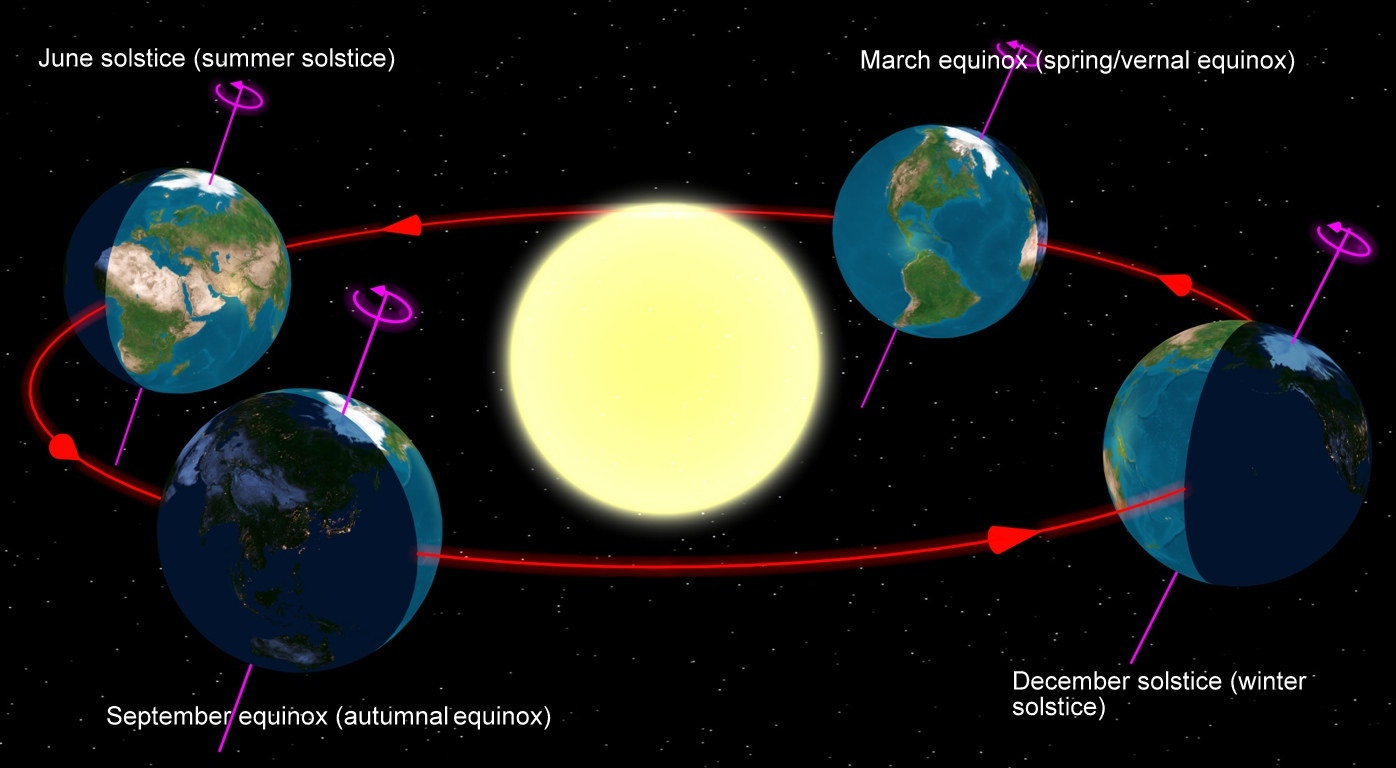
\includegraphics[width=0.8\textwidth]{solstices.jpg}\EC
}

\frame{\frametitle{\textbf{The solstices and equinoxes}}
\Large
\BC
Many cultures have ascribed significance to the annual movement of the Sun. \\

\bigskip
\bigskip

Perhaps the most famous artifact of this is Stonehenge:

\bigskip
\bigskip

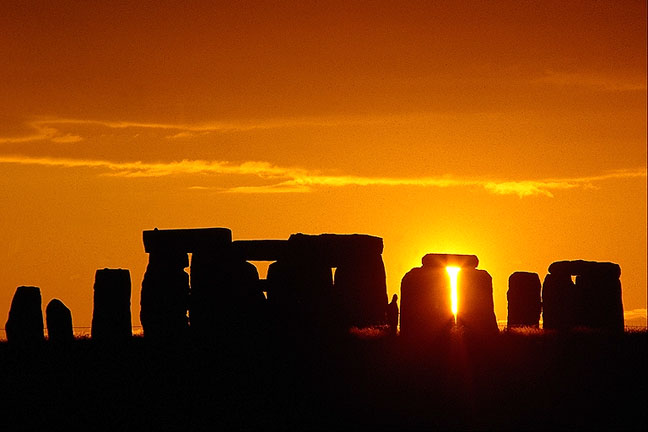
\includegraphics[width=0.6\textwidth]{stonehenge.jpg}

\EC

}



\frame{\frametitle{\textbf{The tropics}}

\BC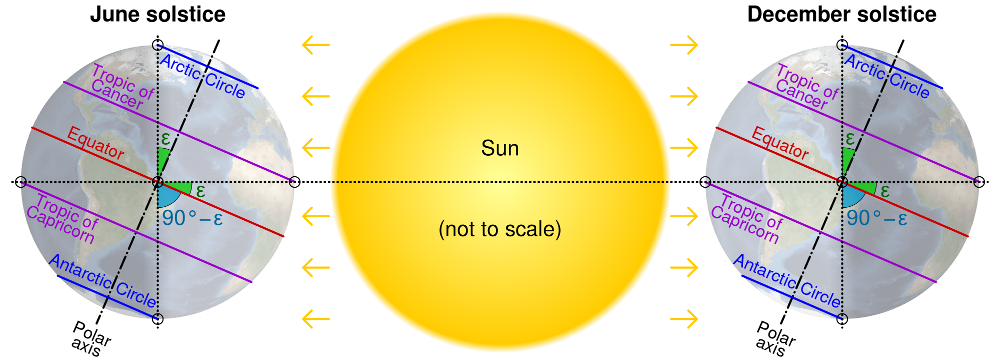
\includegraphics[width=0.6\textwidth]{circle.png}\EC

\bigskip
\bigskip
\bigskip

\Large

The region on Earth where the Sun alternates between the northern sky and the southern sky is called the 
{\color{Red} tropics}.

\bigskip
\bigskip
\large
\BI
\item{The northern boundary is called the {\color{Red}Tropic of Cancer}}
\item{The southern boundary is called the {\color{Red}Tropic of Capricorn}}
\item{These occur at $23.4^\circ$ N/S latitude}
\EI

On the June solstice, the sun reaches the zenith along the Tropic of Cancer.

On the December solstice, the sun reaches the zenith along the Tropic of Capricorn.
}



\frame{\frametitle{\textbf{The Arctic and Antarctic}}

\BC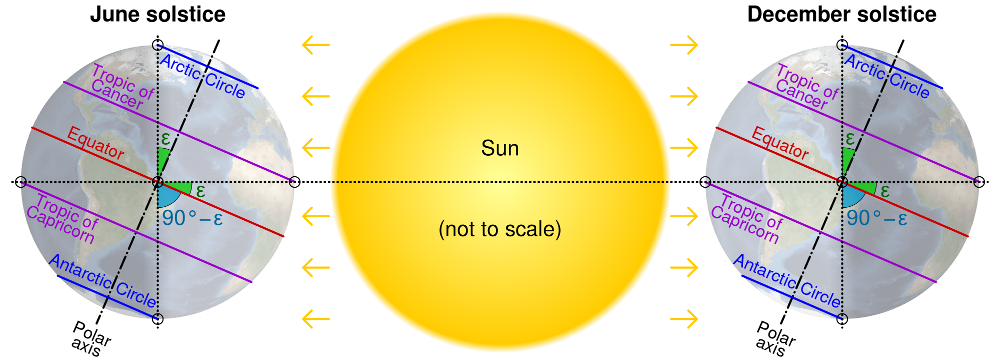
\includegraphics[width=0.6\textwidth]{circle.png}\EC

\bigskip
\bigskip

\Large
The region where the sun either never rises or never sets during part of the year 
is called the Arctic (north) or Antarctic (south).



\bigskip

\BI
\item{North of the Arctic Circle, the sun never rises on the December solstice, and never sets on the June solstice.}
\item{South of the Antarctic Circle, the sun never sets on the December solstice, and never rises on the June solstice.}
\item{These occur at $90-23.4^\circ = 66.6$ N/S latitude}
\EI
}




\frame{\frametitle{\textbf{What consequences does this have on Earth?}}
\Large
Thinking only about noontime (when the sun is highest in the sky), will the sun ever reach the zenith in Syracuse (latitude $43^\circ$ N)?

\bigskip
\bigskip
\bigskip
\bigskip

\color{A}A: Yes \\
\color{B}B: No \\
}

\frame{\frametitle{\textbf{What consequences does this have on Earth?}}
\Large
Thinking only about noontime (when the sun is highest in the sky), will the sun ever reach the zenith in Lima, Peru (latitude $12^\circ$ S)?

\bigskip
\bigskip
\bigskip
\bigskip

\color{A}A: Yes \\
\color{B}B: No \\
}

\frame{\frametitle{\textbf{What consequences does this have on Earth?}}
\Large
Which is true about the Sun on June 21 in Svalbard  (latitude $78^\circ$ N)?

\bigskip
\bigskip
\bigskip
\bigskip

\color{A}A: It will never rise \\
\color{B}B: It will never set \\
\color{C}C: It will reach the zenith of the sky \\
\color{D}D: It will travel from east to west in the northern sky \\
\color{E}E: It will travel from east to west in the southern sky \\
}

\frame{\frametitle{\textbf{The seasons}}
\large
The tilt of the Earth toward/away from the Sun controls the amount of sunlight we get at different times of year!

\bigskip
\bigskip

This happens for two important reasons. Thinking about the Northern hemisphere...

\bigskip
\bigskip

\BI
\item{The Sun is visible in the sky for longer in June than in December}
\item{Sunlight strikes the Earth more directly in June than in December}
\EI

\BC
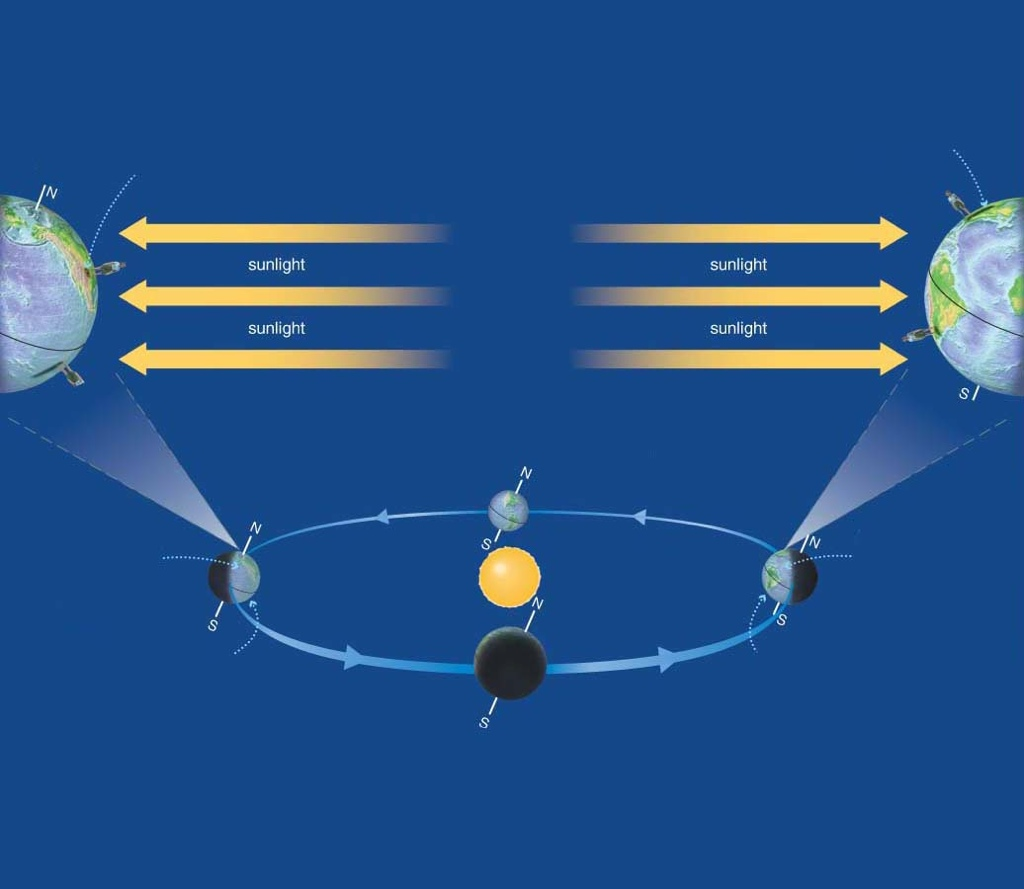
\includegraphics[width=0.5\textwidth]{sun-incidence.jpg}
\EC
}


\frame{\frametitle{\textbf{The seasons}}
\BC
\Huge
Complete Lecture Tutorials pp. 93-98.
\EC
}


\frame{\frametitle{\textbf{The seasons}}
\Large
\BC
This is why the Earth is hotter in summer. \\
It has {\color{Red}nothing} to do with the distance from the Sun!
\EC
}

\frame{\frametitle{\textbf{Exit question}}
\Large
What if the Earth's axial tilt were increased to $30^\circ$ from $23^\circ$?

\bigskip
\bigskip
\bigskip

\color{A}A: Syracuse would have hotter summers \\
\color{B}B: Syracuse would have colder winters \\
\color{C}C: More of Earth would be in the tropics \\
\color{D}D: More of Earth would be in the arctic \\
\color{E}E: Another Stark would meet a bad end \\

\bigskip

\large

Discuss the answer with your neighbors, then write a short explanation down, along with your
NetID or SUID and name, and turn it in on your way out. {\it There may be more than one answer!}
}



\end{document}
